\section{Performance Analysis}
\label{sec:performance}

\subsection{\system{} Overhead}

\begin{figure}[t!]
\centering
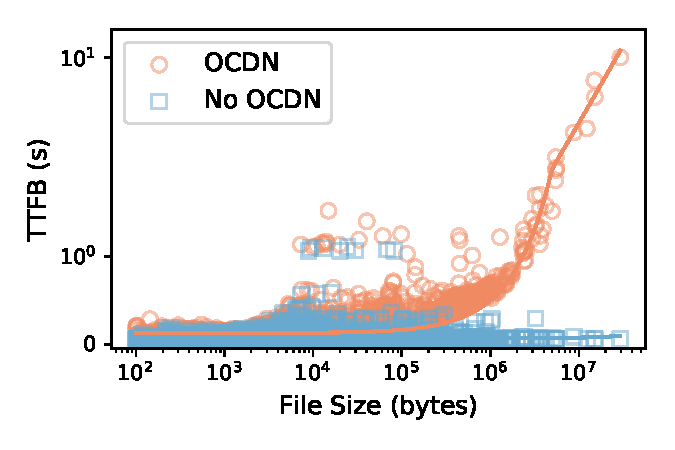
\includegraphics[width=.45\textwidth]{TTFB}
\caption{Time to first byte.}
\label{fig:ttfb}
\end{figure}

\begin{figure}[t!]
\centering
\includegraphics[width=.45\textwidth]{completion}
\caption{Time for completion.}
\label{fig:completion}
\end{figure}

\begin{figure*}[t!]
\centering
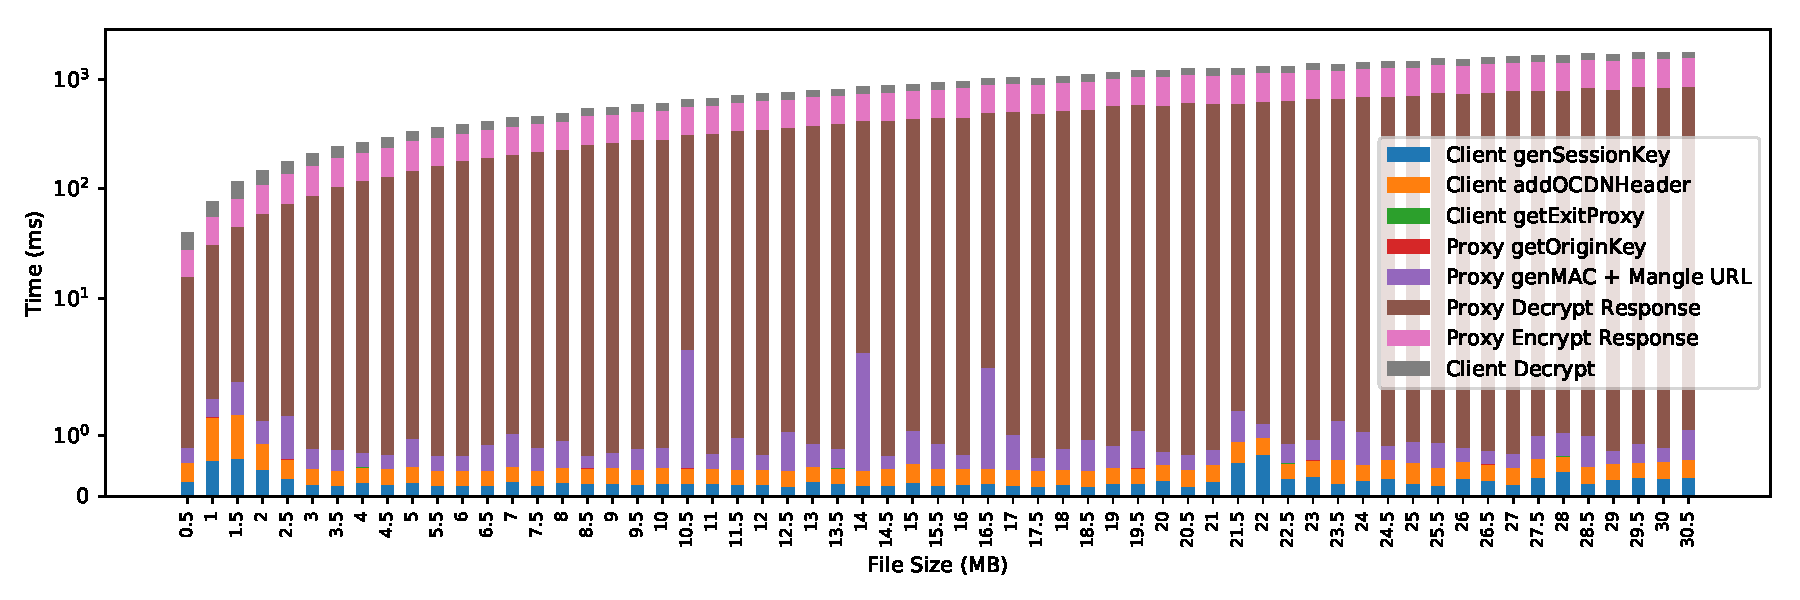
\includegraphics[width=.9\textwidth]{log}
\caption{Overhead of different \system{} operations.}
\label{fig:log}
\end{figure*}

\begin{figure*}[t!]
\centering
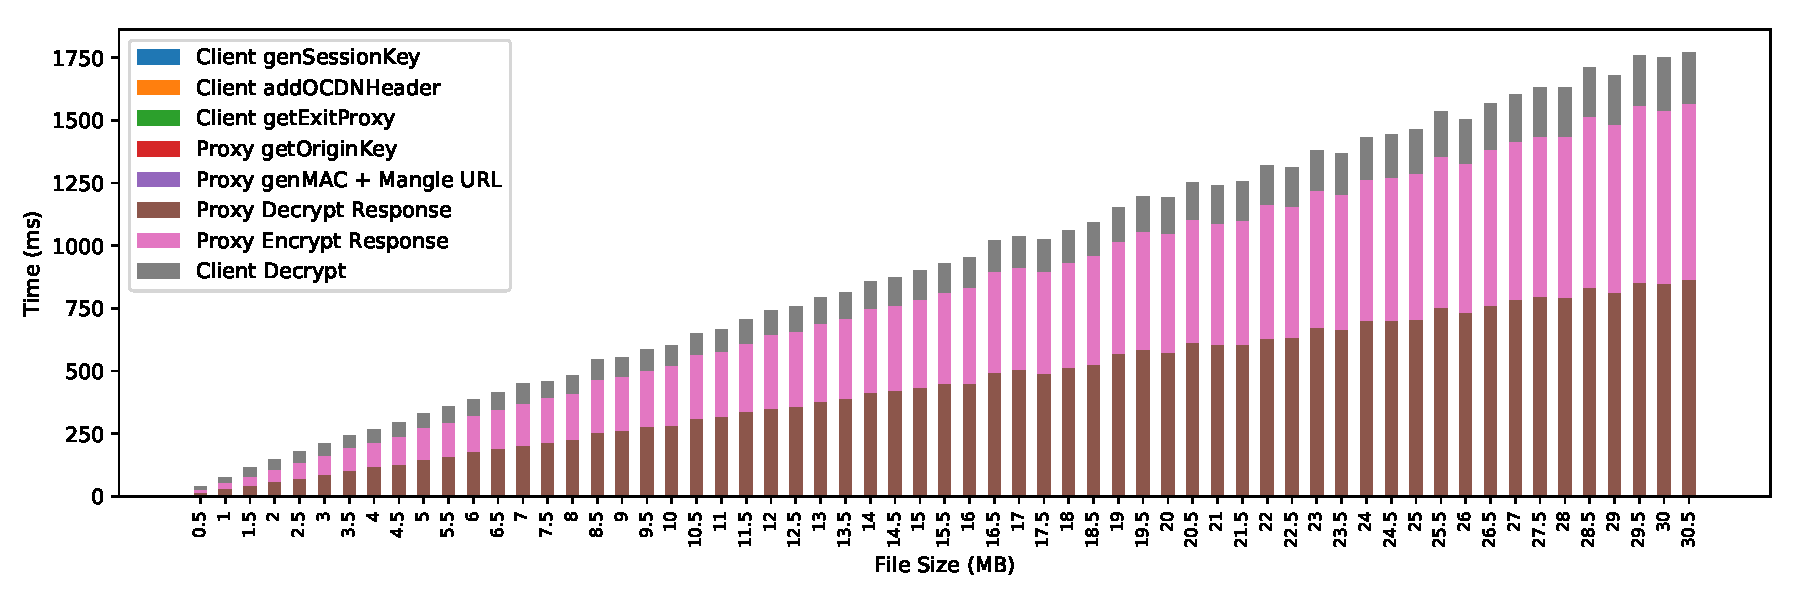
\includegraphics[width=.9\textwidth]{stages}
\caption{Overhead of different stages in \system{}.}
\label{fig:stages}
\end{figure*}

\begin{figure}[t!]
\centering
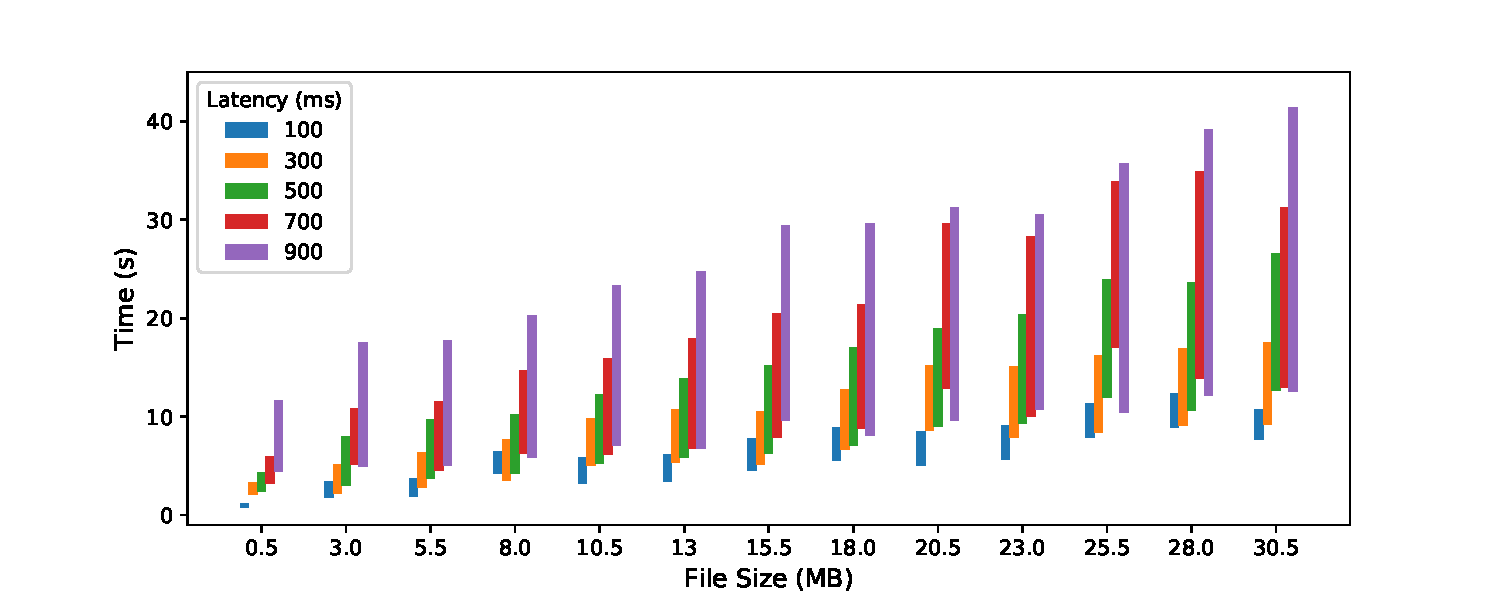
\includegraphics[width=.45\textwidth]{Latency}
\caption{Latency.}
\label{fig:latency}
\end{figure}

\begin{figure}[t!]
\centering
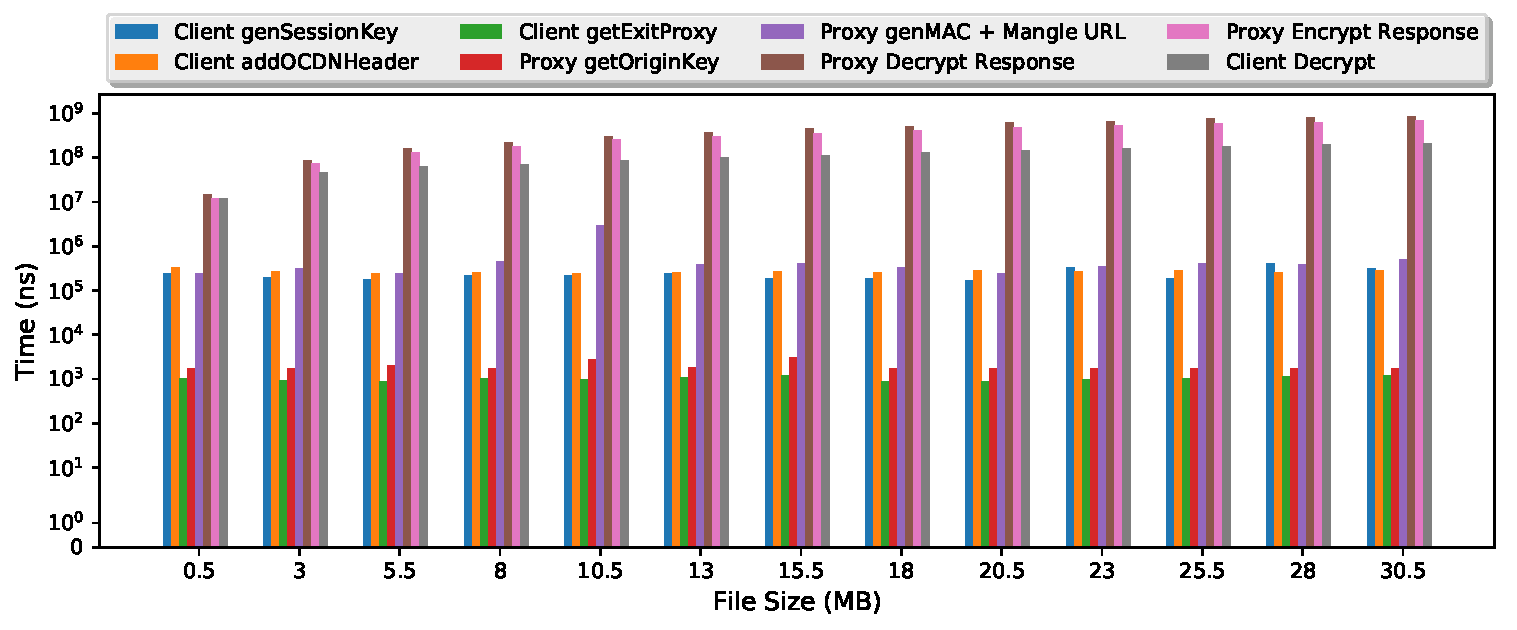
\includegraphics[width=.45\textwidth]{loggrouped}
\caption{Overhead of different operations}
\label{fig:overhead2}
\end{figure}

\subsection{Scalability}
